On peut maintenant décider quelles variables supplémentaires nous ajouterons dans notre modèle. 
La sélection des variables s'est faite de façon assez subjective en analysant les comptes des attributs présentés dans la section \nameref{sec:analyse_prelim} et en ajoutant les attributs qui semblaient avoir le plus grand pouvoir discriminant.
Voici la liste des variables ajoutées:

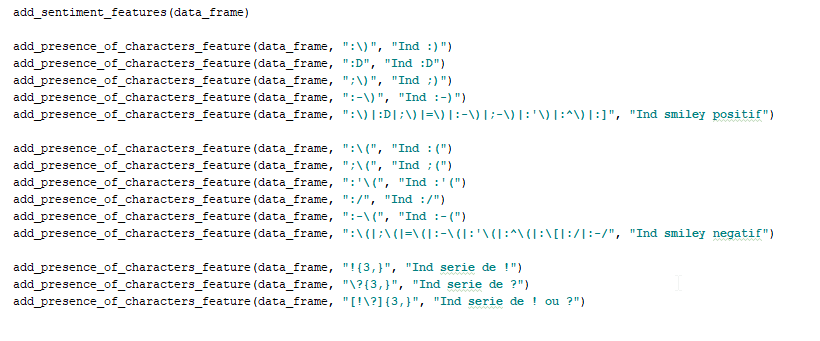
\includegraphics[width=\linewidth,height=14cm]{images/variables_autres}

La fonction \verb|add_sentiment_features| ajoute les 3 variables de sentiments (score de sentiment, nombre de mots positifs et nombre de mots négatifs) et la fonction \verb|add_presence_of_characters_feature| ajoute un 1 si l'expression régulière donnée en argument est trouvée dans l'échange de textos, 0 sinon.
Ainsi, on ajoute des variables de sentiments, des indicateurs de \emph{smileys} positifs et négatifs et des indicateurs de séries de ponctuation à notre jeu de données bruts.
On peut ainsi profiter des données et de l'entraînement de \emph{Senti Word Net} pour ajouter de l'information à nos données avant d'entraîner nos modèles de classification.

En conclusion, lorsqu'on roule le code avec \verb|bool_ajouter_autres_features=True|, on ajoute les variables décrites ci-dessus et on transforme tous les \emph{emojis} en texte qui pourra être capté par les techniques standards de vectorisation des données textuelles.